\section{System Overview}

\indent The overview of the system has been described in Figure~\ref{fig:Overview}. The system has two major components---Camera Module and the Image Processing Unit. The Camera Module consists of the IR camera, Digital camera and the Motor modules. All three modules are controlled by a Raspberry Pi. The motor rotates by a pre-calibrated angle and both the digital and infrared images are taken simultaneously and sent over to a PC where the Image Processing Unit (IPU) is present. The IPU pre-processes images and generates the heat maps from the thermal data. During the training phase the digital images are stitched together and the same stitching mechanism is applied for the IR images during the testing phase. Processed images provide the thermal layout of a wall surface which can then be used to determine leakages and anomalous energy usage.


\begin{figure}[t!]
\begin{center}
	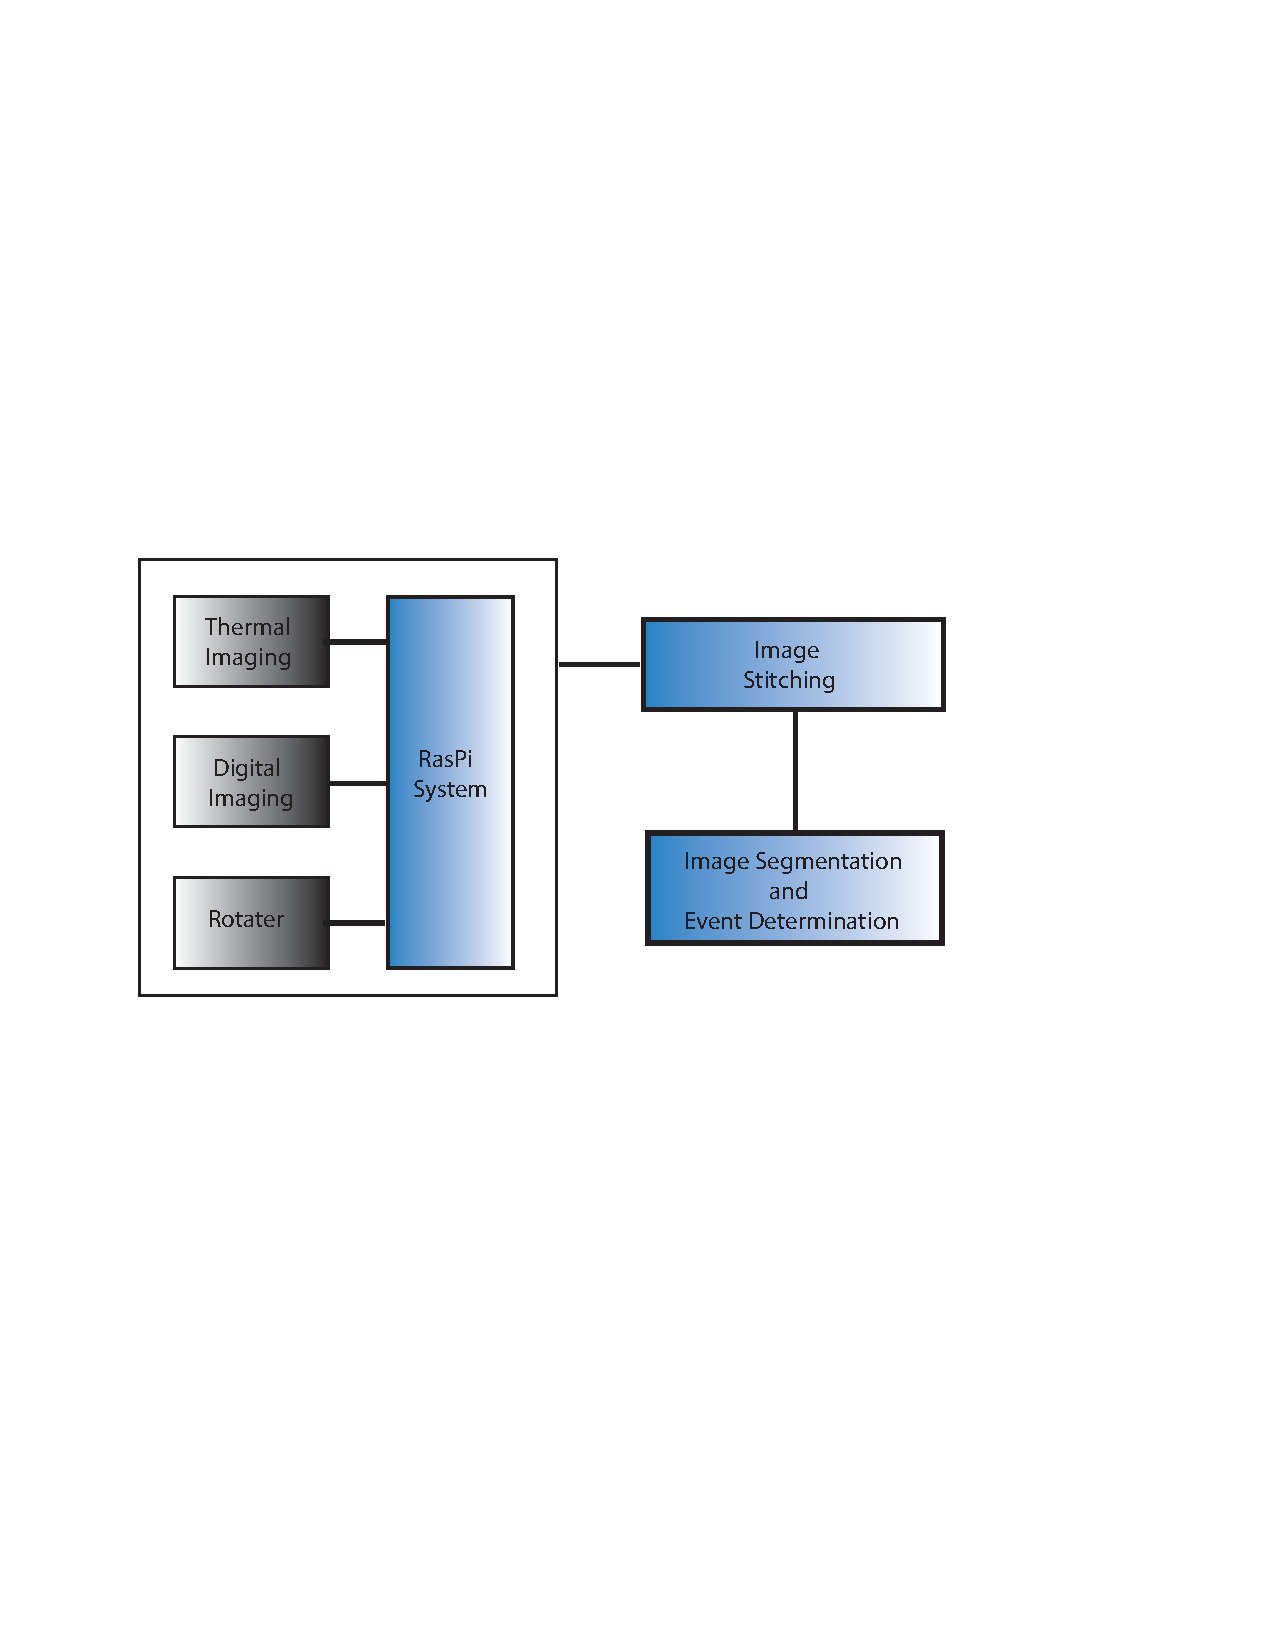
\includegraphics[width=3in]{figs/SystemArch.pdf}
\end{center}
  \caption{Thermal Imaging System Block Diagram}
  \label{fig:Overview}
\end{figure}

\begin{figure}[t!]
	\begin{center}
		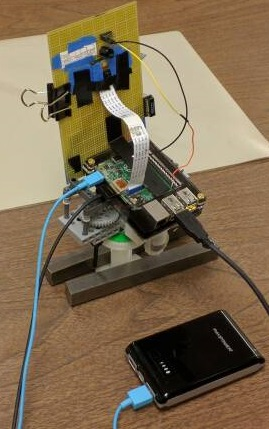
\includegraphics[height=1.5in,width=2in]{figs/SystemDiagram}
	\end{center}
	\caption{IRLeak System}
	\label{fig:SystemDiagram}
\end{figure}